
\frame{
\frametitle{Block-circulant matrices}%此页的标题

\begin{figure}
	\begin{center}
		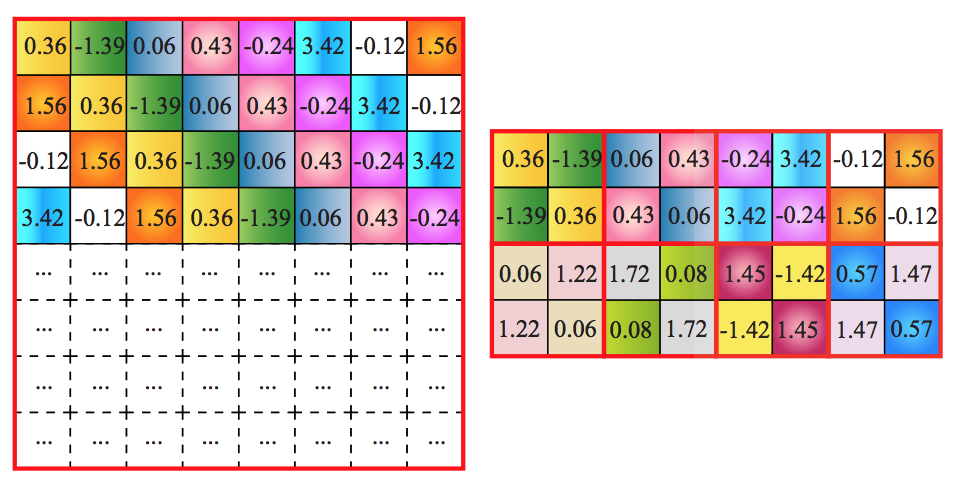
\includegraphics[width=0.8\linewidth]{Picture/block.png}
		\caption{when the numbers of inputs and outputs are not equal}
		\label{Fig:2}
	\end{center}
	% \vspace{-0.1em}
\end{figure}

% \begin{eqnarray}
% 	% a_{5} &=& f\left( W_{51}\cdot X_{1}+W_{52}\cdot X_{2}+W_{53}\cdot X_{3}+W_{54}\cdot X_{4}\right)\\
% 	Y\left( x,y,p\right) =\sum ^{r}_{i=1}\sum ^{r}_{j=1}\sum ^{c}_{c=1}F\left( i,j,c,p\right) X\left( x+i-1,y+j-1,c\right)
% \end{eqnarray}

}